\documentclass{standalone}
\usepackage{preset}
\begin{document}
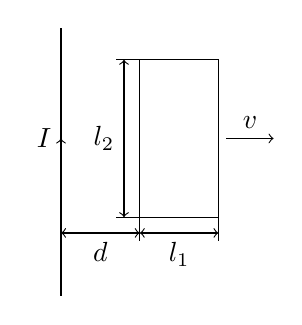
\begin{tikzpicture}[x=20mm,y=20mm]
	\draw[->](-.5,1.2)--(-.5,-.5) (-.5,-.5)--(-.5,.5)node[left]{$I$};
	\draw(0,0)rectangle(.5,1);
	\draw[->](.55,.5)--node[above]{$v$}+(.3,0);
	\draw[<->](-.5,-.1)--node[below]{$d$}(0,-.1);
	\draw[<->](0,-.1)--node[below]{$l_1$}(.5,-.1);
	\draw[<->](-.1,0)--node[left]{$l_2$}(-.1,1);
	\draw(-.15,1)--(0,1) (-.15,0)--(0,0)--(0,-.15) (.5,0)--(.5,-.15);
\end{tikzpicture}
\end{document}
